%slide di introduzione ai fondamenti di Document Type Definition

%frame 01
\begin{frame}
    \frametitle{Elementi per la definizione degli schemi xml}
    \framesubtitle{Principi Document Type Definition}
    \addtocounter{nframe}{1}

    \begin{block}{Esempio DTD}
        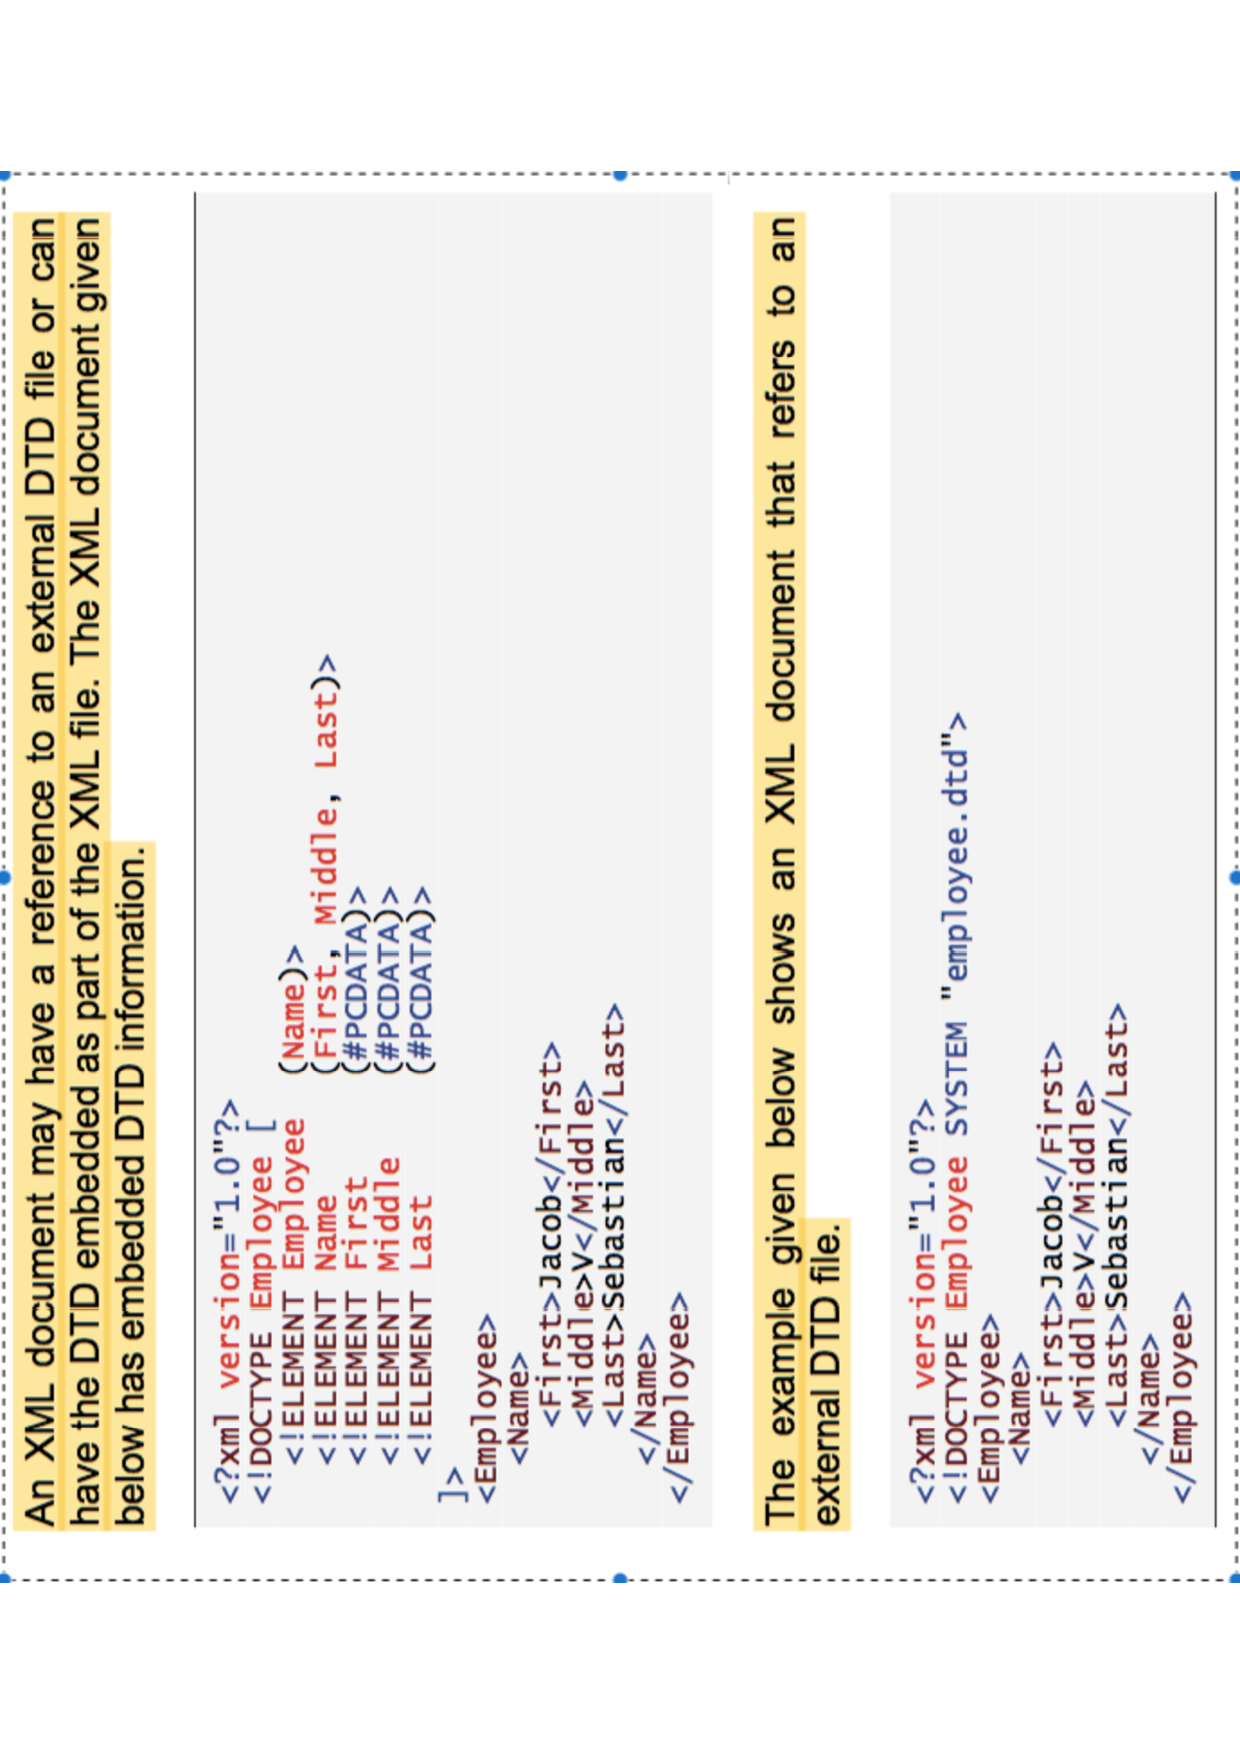
\includegraphics[width=.5\textwidth]{imgs/dtd_1.pdf}
    \end{block}

\end{frame}


\begin{frame}
    \frametitle{Elementi per la definizione degli schemi xml}
    \framesubtitle{Principi Document Type Definition}
    \addtocounter{nframe}{1}

    \begin{block}{Document Type Definition (DTD)}
        A document type definition describes the rule for an xml document structure,
declaring the elements, attributes and entities that are part of the xml
document
    \end{block}

\end{frame}

For an xml document to be valid, it must be well formed and also satisfies the
document type definitions specified by the document type declaration.

included in the document’ prolog

Document validation also aids file sharing since different applications that are
aware of the generally agreed upon document type definition can produce xml
document of similar structure and therefore easily communicate with each
other through data exchange.

any document that lacks a document type declaration may be well formed but
cannot be valid.


following steps:
declare the root element and its children elements

<!ELEMENT element_name (child-element1, child-element-2 ...) >
<!ELEMENT element_name (#PCDATA) >

Parsed character contents are plain texts with no child elements.

Optional modifiers can also be used in element declarations to specify the
number of times a child element may appear.

+ One or more occurrences 
? Zero or one occurrence 
* Zero or more occurrences

If a child element must appear once then leave out the modifier.

<!ELEMENT element_name (B, C)+ >
<!ELEMENT element_name (B+, C) >
<!ELEMENT element_name (B, C+) >
<!ELEMENT element_name (B+, C+) >
If a child element must appear once then leave out the modifier.

A child element declaration is done in the same way as the root element
declaration using the <!ELEMENT > tag

root element declaration must always come first.

Esempio TEI:
- root: TEI
- figli: header - facsimile - text

choice declaration
<!ELEMENT element_name (child_a | child_b) >
indicating a choice of just one, out of the list


Attribute
An attribute is the property of an element that describes the element’s content.

an attribute is declared with <!ATTLIST > element.

<!ATTLIST Element-name Attr-name Attr-type Attr-state? default-value? >

``Element-name'' is the name of the element
``Attr-name'' is the attribute to be declared.
``Attr-type'' specifies the expected attribute’s data type
The Attr-state denota una tra i tre stati possibili di un attributo 
``default-value'' if provided is the value to be used if the attribute is not
supplied

TABELLA dei tipi

The state can be any of #IMPLIED (an optional attribute), #REQUIRED (a compulsory attribute) or #FIXED (a fixed value
attribute that may not be changed) the value is provided as the default value. You cannot use the default-value with the #REQUIRED state as you must
supply a value for the attribute.

Esempio:
root: TEI
figli: header(obbligatorio una volta sola) - facsimile(opzionale una volta sola) - testo(obbligatorio una o più volte)
attributi: 
- header: type:(fixed, CDATA ``intestazione''); lang(opzional, NMTOKEN)
- facsimile: source:(obbligatorio)
- testo: id(obbligatorio, contenuto id) type(opzionale contenuto testuale)

MIXED CONTENT
The declaration syntax for mixed content is as follows: <!ELEMENT
element_name (#PCDATA|child_element)* >

Empty elements 
the only difference is that the child element name is
substituted with the keyword “EMPTY” like this <!ELEMENT element_name
EMPTY>

Any Element
The content specification “ANY” when used in a declaration implies that any
element as well as texts can be the child or content of the declared element.
The syntax of usage for content specification “ANY” is as described below:
<!ELEMENT element_name ANY >

Esercizio: includere all'interno di un documento XML la dichiarazione del tipo.

The document type declaration contains or points to the location of the
document type definition.

The document type declaration is placed in the xml document prolog; between
the xml declaration and the root element.

<!DOCTYPE root_element SYSTEM “External DTD’s URL“ [
Internal DTD ]>

<!DOCTYPE root_element [Internal DTD] >
<!DOCTYPE root_element SYSTEM “External_DTD’s URL” >
re-usability reasons, and then link it to the xml document and any other xml
document through its URL

Esercizio: inserire all'interno di un file XML la dichiarazione degli elementi del documento istanziare un documento valido.
Alla fine creare un file esterno con estensione .dtd e includerlo nel prologo XML.


ENTITY:


An xml document may include other xml documents and data from different
sources, these sources are termed entities and an entity can be external or
internal entity.


Internal general entities help include special characters in an xml document,
that would otherwise make an xml document become malformed if included
literally.


The syntax of usage is as described below:


https://leggi.amazon.it/notebook?ref_=kcr_notebook_lib
18/4410/3/2018
Kindle: Your Notes and Highlights
<!ENTITY entity_name “replacement_string” or “hexadecimal_code” >


To use the entity name in the element content simply attach the ampersand to
the beginning of the entity name and append the semi colon to the end like
this; &entity_name;


may include well formed xml elements.


An xml document may be developed from other xml document located in
different places and from different applications. This is made possible through
the use of external general entities. Through which the external entities are
inserted into the main xml document. The syntax for an external general entity
is as described below: <!ENTITY entity_name SYSTEM “URL” > The URL
points to the location of the external entity to be drawn into the main
document.


<!ENTITY External_fruits SYSTEM "fruits.xml" >


Please note that an external entity cannot contain a document type declaration
as it will conflict with the main xml document type declaration, but you may
include a text declaration in an external parsed entity, if not the parser will
naturally assume a “UTF-8” encoding for the external entity. General entities
though declared in the DTD, must be used in the document and not in the
DTD itself. Also for now, Mozilla, Netscape, Safari and Opera do not resolve
entity references except the latest version of internet explorer.


https://leggi.amazon.it/notebook?ref_=kcr_notebook_lib
19/4410/3/2018
Kindle: Your Notes and Highlights
General entities defined in the document type definition must appear in the xml
document content, becoming a part of the xml document. This is a limitation of
general entities as they cannot be exclusively used as parameters in the
document type definition.


This is however addressed by parameter entities. Parameter entity usage
syntax is as described below: <!ENTITY % entity_name “replacement_string”
>


In other words parameter entity references are part of the DTD but may not
appear in the document content.


More, a parameter entity reference is started with a percentage sign


(%) and not with the ampersand, and terminated with a semi colon like shown
below: %parameterEntityName;


There are two types of parameter entity; the internal and the external
parameter entities.


Internal parameter entities are used much in the same way that the general
entity references are used but they remain parts of the dtd and never appear
in the document’s content. An internal parameter entity reference is
represented as shown below: <!ENTITY % parameter_entity_name
“replacement_content” >
Note:
https://leggi.amazon.it/notebook?ref_=kcr_notebook_lib
20/4410/3/2018
Kindle: Your Notes and Highlights
Yellow highlight | Location: 786
When a parameter entity is inserted in the dtd, the parameter entity is replaced
with the replacement content at execution time.


Internal parameter entities are declared in the dtd external subset


This would make the dtd easier to develop and later maintained, if there are
any changes to be made.


A parameter entity that is only a part of a complete declaration like above
cannot appear in the internal definition subset of a dtd and must be placed in
the external definition subset and referred to.


Note that the parameter entity reference ”%Event_info;” was declared before it
was used, and that “sport_calendar.dtd” was referred to in the external dtd
subset as described in document 5.3 below:


External parameter entities enable the modularization and linking of document
type definitions.


with external parameter entities you can embed modularized document type
definitions from different locations to form a single and more complete
document type definition.
Note:
https://leggi.amazon.it/notebook?ref_=kcr_notebook_lib
21/4410/3/2018
Kindle: Your Notes and Highlights
Yellow highlight | Location: 876
The syntax for an external parameter entity is as described below:


<!ENTITY % parameter_name SYSTEM “URL” > %parameter_name;


using an external parameter entity reference as shown
